\documentclass{article}

% -------------------------------------------------
% Packages
% -------------------------------------------------

\usepackage{xcolor}
\usepackage{amsmath}
\usepackage{amssymb}
\usepackage{amsthm}
\usepackage{graphicx}
\usepackage{subcaption}
\usepackage{matlab-prettifier}
\usepackage{listings}
\usepackage{blindtext}
\usepackage{geometry}
\usepackage{float}
\usepackage{dirtytalk}
\usepackage{enumitem}
\usepackage{derivative}
\usepackage{biblatex}
\usepackage{svg}
\usepackage{hyperref}
\usepackage{pgfplots}
\pgfplotsset{compat=1.18}

% -------------------------------------------------
% Colors
% -------------------------------------------------

\definecolor{darkgreen}{rgb}{0.0, 0.5, 0.0}

% -------------------------------------------------
% Hyperlinks
% -------------------------------------------------

\hypersetup{
    colorlinks=true,
    linkcolor=blue,
    citecolor=blue,
    urlcolor=blue
}

% -------------------------------------------------
% Theorem environments
% -------------------------------------------------

% Numbered
\newtheorem{theorem}{Theorem}[section]
\newtheorem{lemma}[theorem]{Lemma}
\newtheorem{proposition}[theorem]{Proposition}

% Unnumbered
\newtheorem*{theorem*}{Theorem}
\newtheorem*{lemma*}{Lemma}
\newtheorem*{proposition*}{Proposition}

\theoremstyle{definition}
\newtheorem{definition}[theorem]{Definition}
\newtheorem{example}[theorem]{Example}

\theoremstyle{remark}
\newtheorem{remark}[theorem]{Remark}

% -------------------------------------------------
% Equation numbering
% -------------------------------------------------

% Reset equation numbering at each subsection
\makeatletter
\@addtoreset{equation}{subsection}
\makeatother

% If you want equations to be numbered by subsection,
% uncomment the following line:
% \renewcommand{\theequation}{\thesubsection.\arabic{equation}}

% -------------------------------------------------
% Python / MATLAB code formatting
% -------------------------------------------------

\lstset{
    language=Python,
    basicstyle=\ttfamily\small,
    keywordstyle=\color{blue},
    stringstyle=\color{darkgreen},
    commentstyle=\color{gray},
    showstringspaces=false,
    frame=single,
    numbers=left,
    numberstyle=\tiny\color{gray},
    breaklines=true
}

% -------------------------------------------------
% Page geometry
% -------------------------------------------------

\geometry{
    a4paper,
    total={160mm,250mm},
    left=25mm,
    top=30mm,
    footskip=10mm
}

% -------------------------------------------------
% Document settings
% -------------------------------------------------

\setlength{\parindent}{0pt}

% -------------------------------------------------
% Title
% -------------------------------------------------

\title{Calculus Uge 1}
\author{Thomas Sejer Canham}
\date{\today}

% =================================================
% Document
% =================================================

\begin{document}

% -------------------------------------------------
% Title page
% -------------------------------------------------

\begin{titlepage}

    \maketitle
    \thispagestyle{empty}

\end{titlepage}
Vi skal i denne uge kigge på de gængse regneregler for differentiation, og vi skal se på hvordan man kan bruge dem til. Ydermere skal vi berøre extreme value theorem. Vi skal også kigge lidt på fundamental integration, dvs. hvordan helt normalt integraler kan beregnes. 
\section*{Gængse begreber til uge 1}
Det vil allerede nu være nyttig at bemærke at "prime" notationen er kort notation for differential operatoren
 $$\frac{d}{dx}.$$ For eksempel er $f'(x) = \frac{df}{dx}$, og $f''(x) = \frac{d^2f}{dx^2}$ Dette vil vise sig nyttigt senere i kurset. Det hyppigst brugte regneregler for differentiation er:

\begin{itemize}
    \item Kædereglen: $f(g(x))' = f'(g(x))  g'(x)$, eller $(f \circ g)' = f'(g(x))  g'(x)$
    
    \item Produktreglen: $(f(x)  g(x))' = f'(x)  g(x) + f(x)  g'(x)$

    \item Kvotientreglen: $\left(\dfrac{f(x)}{g(x)}\right)' = \dfrac{f'(x)  g(x) - f(x)  g'(x)}{(g(x))^2}$
\end{itemize}
Derudover er det nyttigt at bemærke at differentiation er en lineær operator, hvilket betyder at
$$\frac{d}{dx}(f(x) + g(x)) = f'(x) + g'(x)$$
og at for en constant $c \in \mathbb{R}$
$$\frac{d}{dx}(c f(x)) = c  f'(x)$$
Sammensat giver dette os at
$$\frac{d}{dx}c( f(x) + g(x)) = c  f'(x) + c g'(x)$$

Hyppigt vil det også være nyttigt at bruge nulreglen. Lad $f(x)$ være en vilkårlig funktion. Så er 
$$f(x)\cdot x = 0$$
hvis og kun hvis $f(x) = 0$ eller $x = 0$. Dette er nyttigt når man skal finde kritiske punkter, da man ofte vil ende med et produkt af funktioner, og man kan så bruge nulreglen til at finde de kritiske punkter.\vspace{.5cm}
Jeg vil også minde jer om at for et vilkårligt andengradspolynomium $ax^2 + bx + c$ er rødderne givet ved kvadratsætningen:
$$x = \frac{-b \pm \sqrt{b^2 - 4ac}}{2a}$$

\section*{Den afledte test}
Lad $c$ være et tal i intervallet $ I = (a,b)$, og lad $f$ være en funktion der er differentiabel på $(a,b)$. Hvis $f'(x) > 0$ for alle $x \in (a,c)$, og $f'(x) < 0$ for alle $x \in (c,b)$, så har $f$ et lokalt maksimum i $c$. \vspace{1em}

 Hvis $f'(x) < 0$ for alle $x \in (a,c)$, og $f'(x) > 0$ for alle $x \in (c,b)$, så har $f$ et lokalt minimum i $c$.

 \section*{Extreme Value Theorem (EVT)}
 Jeg vil nu definerer Extreme Value Theorem og beskrive det nærmere.

\begin{theorem*}[Extreme Value Theorem]
    Lad $[a,b]$ være et lukket interval, og lad
    $f:[a,b]\to\mathbb{R}$ være en kontinuert funktion.
    Da antager $f$ både et maksimum og et minimum på intervallet.
\end{theorem*}
Hvis vi er lidt mere restriktive og lader $f$ være differentiabel på intervallet, så ved vi at maksimalværdien eller minimal værdien må findes i:
\begin{enumerate}
    \item De kritiske punkter, dvs. $x$ hvor $f'(x) = 0$
    \item Intervalendepunkterne, dvs. $f(a)$ eller $f(b)$
\end{enumerate}
(Denne udvidelse kaldes Fermats Theorem on Stationary Points)

\section*{Opgave 6.2 9.}
Vi bliver givet en funktion
\begin{equation}
    N(t) = 20 (\dfrac{t}{12} - \ln(\dfrac{t}{12} )) + 30
\end{equation}
der beskriver antallet af bakterier pr mililiter vand som en funktion af tiden $t$ i dage. Funktionen er defineret i intervallet [1,15]. Bemærk at vi er givet en differentiabel funktion på et lukket interval og kan brugt extreme value theorem. \vspace{1em}
Vi finder først den afledte funktion $N'(t)$:
\begin{align*}
N'(t) &= \frac{d}{dt} \left( 20 (\dfrac{t}{12} - \ln(\dfrac{t}{12} )) + 30 \right) \\
&= 20 \left( \frac{1}{12} - \frac{1}{t} \right) \\
&= \frac{20}{12} - \frac{20}{t}
\end{align*}
Bemærk at $\ln(\dfrac{t}{12}) = \ln(t) - \ln(12)$. Det ses at $N'(t)$ er defineret for alle $t \in [1,15]$. For at finde kritiske punkter, sætter vi $N'(t) = 0$, og finder at
$$\frac{20}{12} - \frac{20}{t} = 0 \iff t = 12.$$

Vi indsætter nu det kritiske punkt og intervalendepunkterne i $N(t)$ for at finde de tilhørende værdier:
\begin{align*}
N(1) &= 20 (\dfrac{1}{12} - \ln(\dfrac{1}{12} )) + 30 \approx 81.4 \\
N(12) &= 20 (\dfrac{12}{12} - \ln(\dfrac{12}{12} )) + 30 = 50 \\
N(15) &= 20 (\dfrac{15}{12} - \ln(\dfrac{15}{12} )) + 30 \approx 50.5
\end{align*}

Det vil sige at a) funktionen minimeres i $t = 12$ med b) $N(12) = 50$ og maksimeres i c) $t = 1$ med d) $N(1) \approx 81.4$.

\begin{figure}[H]
    \centering
    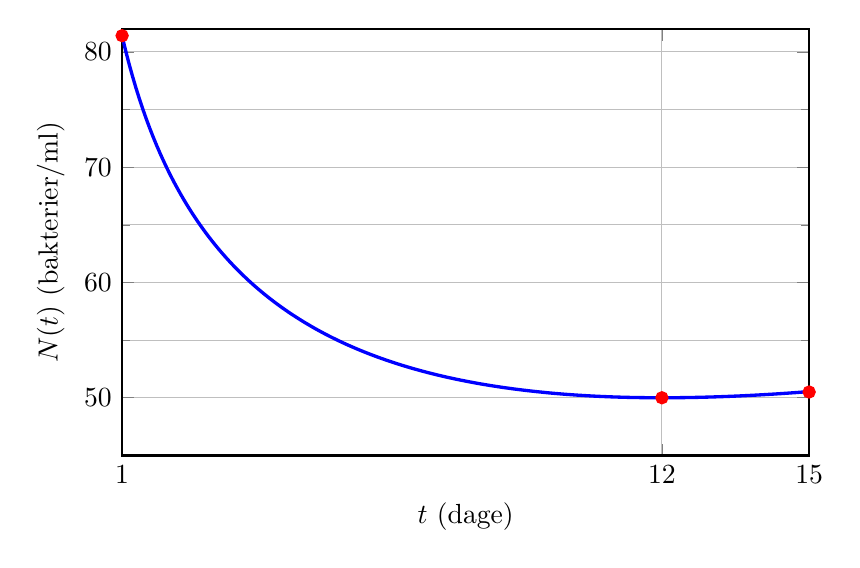
\begin{tikzpicture}
        \begin{axis}[
            width=0.85\textwidth,
            height=7cm,
            xlabel={$t$ (dage)},
            ylabel={$N(t)$ (bakterier/ml)},
            xmin=1, xmax=15,
            ymin=45, ymax=82,
            xtick={1,12,15},
            ytick={50,60,70,80},
            grid=both,
            minor tick num=1,
            thick,
        ]
            \addplot[blue, very thick, domain=1:15, samples=200]
                {20*(x/12 - ln(x/12)) + 30};
            \addplot[only marks, mark=*, mark size=2pt, red]
                coordinates {(1,81.4) (12,50) (15,50.5)};
        \end{axis}
    \end{tikzpicture}
    \caption{Grafen for $N(t)$ på intervallet $[1,15]$.}
\end{figure}


\newpage
\section*{Opgave 5.2 54}
Vi bliver givet en funktion $D(x) = -x^4 +8x^3 + 80x^2$ der beskriver  ændring i folks holdninger som en funktion af $x$, hvor $x$ er diskrepansen mellem lytter og taler. Vi vil gerne finde den værdi af $x$ der maksimerer $D(x)$.

Vi finder først den afledte funktion $D'(x)$:
\begin{align*}
D'(x) &= \frac{d}{dx}(-x^4 + 8x^3 + 80x^2) \\
&= -4x^3 + 24x^2 + 160x
\end{align*}
For at finde kritiske punkter, sætter vi $D'(x) = 0$:
\begin{align*}
-4x^3 + 24x^2 + 160x &= 0 \\
-4x(x^2 - 6x - 40) &= 0
\end{align*}
Dette giver os to løsninger: $x = 0$ og løsningerne til kvadratet $x^2 - 6x - 40 = 0$. Vi kan bruge kvadratsætningen $x = \frac{-b \pm \sqrt{b^2 - 4ac}}{2a}$ til at finde de resterende løsninger:
\begin{align*}
x &= \frac{6 \pm \sqrt{(-6)^2 - 4(1)(-40)}}{2(1)} \\
&= \frac{6 \pm \sqrt{36 + 160}}{2} \\
&= \frac{6 \pm \sqrt{196}}{2} \\
&= \frac{6 \pm 14}{2} = -4 \vee  10
\end{align*}
Vi har nu tre kritiske punkter: $x = -4$, $x = 0$, og $x = 10$. For at bestemme hvilke af disse punkter der giver et lokalt maksimum, kan vi bruge den afledte test. Vi undersøger fortegnet af $D'(x)$ omkring de kritiske punkter.
For $x < -4$, vælger vi $x = -5$:
\begin{align*}
D'(-5) &= -4(-5)^3 + 24(-5)^2 + 160(-5) > 0
\end{align*}
For $-4 < x < 0$, vælger vi $x = -1$:
\begin{align*}
D'(-1) &= -4(-1)^3 + 24(-1)^2 + 160(-1) < 0
\end{align*}
Og finder at $x=-4$ er et lokalt maksimum. \vspace{1em}

For $0 < x < 10$, vælger vi $x = 1$:
\begin{align*}
D'(1) &= -4(1)^3 + 24(1)^2 + 160(1) > 0
\end{align*}
Dermed er $x=0$ et lokalt minimum. \vspace{1em}
For $x > 10$, vælger vi $x = 11$:
\begin{align*}
D'(11) &= -4(11)^3 + 24(11)^2 + 160(11) < 0
\end{align*}
Og finder at $x=10$ er et lokalt maksimum. \vspace{1em}

Vi kan så indsætte de kritiske punkter i $D(x)$ for at finde de tilhørende værdier:
\begin{align*}
D(-4) &= -(-4)^4 + 8(-4)^3 + 80(-4)^2 = 256 - 512 + 1280 = 1024 \\
D(0) &= -(0)^4 + 8(0)^3 + 80(0)^2 = 0 \\
D(10) &= -(10)^4 + 8(10)^3 + 80(10)^2 = -10000 + 8000 + 8000 = 5000
\end{align*}

\end{document}
